% Experiment 5: backend/evals/paper/exp5_farming.py
We built rating histories for several attackers and passed them through the
production profile builder and farming detectors. The benchmark is an honest runner
rated five stars by twenty strangers, whose ranking score is 4.57. An honest runner
rated by twenty strangers (mostly five stars) and five friends scores 4.52, so a
normal share of friends among one's customers costs nothing.

Fig.~\ref{fig:farming}(a) follows a runner who served six strangers badly (mean 3.0),
was penalised, and then collected five-star ratings from three friends. The plain
average climbs to 4.96. Weighting each rating, which is how the system worked before
it moved to one vote per rater, lets the farmed score pass the honest benchmark at
160 ratings. The deployed weighting stays between 3.21 and 3.65 however many ratings
are farmed, because three friends remain three votes and their weight falls as their
share of the history grows. With eight friends the deployed score peaks at 3.83. On
the ranking scale of~\eqref{eq:effective}, this is the difference between the honest
runner's 857~m advantage and at most 263~m for the farmer. The farming detectors
flagged every history with 20 or more farmed ratings, whether the runner had been
penalised or was farming from a standing start.

The breadth attack (Fig.~\ref{fig:farming}(b)) is the limit. If every farmed rating
comes from a different
friend, one rating each, one vote per rater gives no protection: eighty such friends
reproduce the honest benchmark of 4.57 exactly, and none of the three detectors fires
because no friend rates twice and there is no stranger to compare against. The attack
needs eighty real, verified accounts that have accepted a friend request and each paid
for a real errand, and friendship maturity (Section~\ref{sec:design-trust}) makes the
new ties count for less in trust, though not in reputation. We do not defend against
it beyond that cost.

\begin{figure}[!t]
\centering
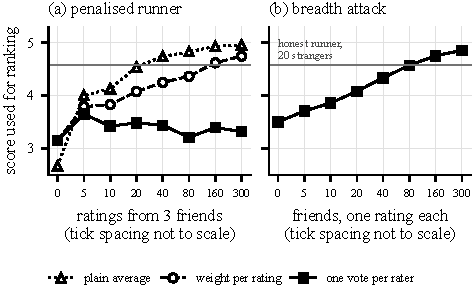
\includegraphics[width=\columnwidth]{figures/fig_farming.pdf}
\caption{(a) Ranking score of a penalised runner as three friends add five-star
ratings, under three weightings. (b) The breadth attack under the deployed weighting,
in which each rating comes from a different friend. The horizontal axes are
categorical and roughly doubling, not linear. The histories are constructed, not
sampled, so there is no seed variation to show.}
\label{fig:farming}
\end{figure}
